\documentclass[12pt]{article}
\usepackage{graphicx}
\usepackage{hyperref}
\usepackage{eso-pic} 
\usepackage{lipsum} 
\usepackage{amsmath}
\usepackage{listings}
\usepackage{amsmath}
\usepackage[linesnumbered,ruled, longend]{algorithm2e}
\usepackage{tikz}
\usepackage{tabularx}
\usepackage{colortbl}
\usepackage{fancyhdr}
\usepackage{float}
\usepackage{xcolor}
\usepackage[T1]{fontenc}

\usetikzlibrary{shapes.geometric, arrows}
\tikzstyle{node} = [rectangle, rounded corners, minimum width=1cm, minimum height=1cm,text centered, text width=3cm, draw=black, fill=red!30]
\tikzstyle{level1} = [rectangle, rounded corners, minimum width=1cm, minimum height=1cm, text centered,text width=3cm, draw=black, fill=orange!30]
\tikzstyle{level2} = [rectangle, rounded corners, minimum width=1cm, minimum height=1cm, text centered,text width=3cm, draw=black, fill=green!30]
\tikzstyle{level3} = [rectangle, rounded corners, minimum width=1cm, minimum height=1cm, text centered,text width=1.5cm, draw=black, fill=blue!30]
\tikzstyle{arrow} = [thick,->,>=stealth,blue]
\tikzset{edge from parent path={ (\tikzparentnode) -- +(0,-20pt) -| (\tikzchildnode)}}
\setlength{\parindent}{0em}
\setlength{\parskip}{1em}
\definecolor{pblue}{rgb}{0.13,0.13,1}
\definecolor{pgreen}{rgb}{0,0.5,0}
\definecolor{pred}{rgb}{0.9,0,0}
\definecolor{backcolour}{rgb}{0.95,0.95,0.92}
\lstset{language=Java,
	backgroundcolor=\color{backcolour},
	commentstyle=\color{pgreen},
	keywordstyle=\color{pblue},
	stringstyle=\color{pred},
	basicstyle=\ttfamily,
	numbers=left,
	numberstyle=\tiny,
	frame=single,
	title=\lstname
}

\definecolor{bluepale}{RGB}{10,120,155}
%---------------------------------------------


\title{- Rapport  - \\Projet 2 \\ \textbf{Jeu de Hex et bandits manchots} }
\author{ Amadou Bah\\ Celestin Mireux \\Daouda TRAORE \\  Junior MISSOUP}
\renewcommand*\contentsname{Table des matières}
\date{}
\begin{document}
\AddToShipoutPicture*
{\put(440,650){
\includegraphics[width=6cm,height=6cm]{images/logo.jpg}}}
\maketitle
\mbox{}
\vfill
L3 Informatique 2022-2023 Université Caen Basse-Normandie.


\tableofcontents

\newpage
\section{Introduction}	
Pour l'évaluation de la matière projet2 qui a pour but de nous inculquer les meilleures attitudes et compétences de programmation il nous a été proposé multiples sujets pour nous évaluer afin de mettre en pratique nos connaissances et nos compétences. Parmi tous ces sujets celui qui nous ont le plus Intéressé fut la coloration IA : Jeu d'Hex et bandits manchots. Ce jeu n'est pas très different de jeu qu'on a eu à réaliser mais la stratégie appliquée a ce jeu pour gagner une partie est un peu de différente, quand on parle de stratégie du point de vue d'une machine c'est l'algorithme qu'elle va utilider pour gagner une partie. On sait que les jeux extensifs, comme hex, le go ou les échecs, peuvent se représenter sous la forme d'arbre, et que l'essentiel du travail pour gagner est de prédire un score pour chaque nœud. Pour faire ça on analyse toutes les possibilités du jeu, ou on utilise des fonctions d'évaluation qui permet d'approximer l'état du jeu. Mais c'est méthodes peuvent avoir des limites.

Parmi ses limites, on a vu que certains jeux n'ont pas de fonctions d'évaluation évidentes et quand il y a trop de coups possibles, l'arbre de recherche devient beaucoup trop grand ce qui rend le temps de calcul d'un meilleur coup très long.
C'est pourquoi pour ce projet, on va donc essayer de voir une autre méthode qui permette de traiter ces deux cas. 
Mais on est dans une situation pour le moins complexe : quelle que soit la profondeur à laquelle on ira chercher notre meilleur, nous n'avons pas de fonction d'évaluation, il nous sera impossible d'évaluer notre plateau.

Il va donc nous falloir trouver une autre solution. Il existe déjà un algorithme intéressant pour faire des estimations sur la valeur d'un coup sans avoir besoin d'évaluer le plateau, qui s'appelle \textbf{Monte-Carlo Tree search}.

Ce projet nous a donc amené à travailler sur des connaissances qui sont nouvelles pour nous, que ce soit les  algorithmes de résolution ou encore des choses complexes du développement des applications. Ce rapport a pour objectif de présenter comment nous avons travaillé et quels ont été les multiples obstacles que nous avons dû faire face.
	\\
Le présent rapport est organisé en trois grandes parties. La première est consacrée à la présentation du jeu, puis nous parlerons de la répartition des tâches, du développement du moteur, de l'implementation de MCTS  et enfin de la création  de l'interface graphique et des problèmes rencontrés.
\newpage
\section{\underline{Histoire et règle de l’hex}}

	Inventé en 1942 par le poète et physicien danois Piet Hein, le jeu d'Hex est un jeu de stratégie abstrait, comme les échecs et le Go, par exemple.

    Il est redécouvert, en 1948, par le célèbre économiste et mathématicien américain John Forbes Nash. Depuis, il a  fasciné de nombreux amateurs de jeux combinatoires.  

\begin{figure}[h!]
	\begin{center}
		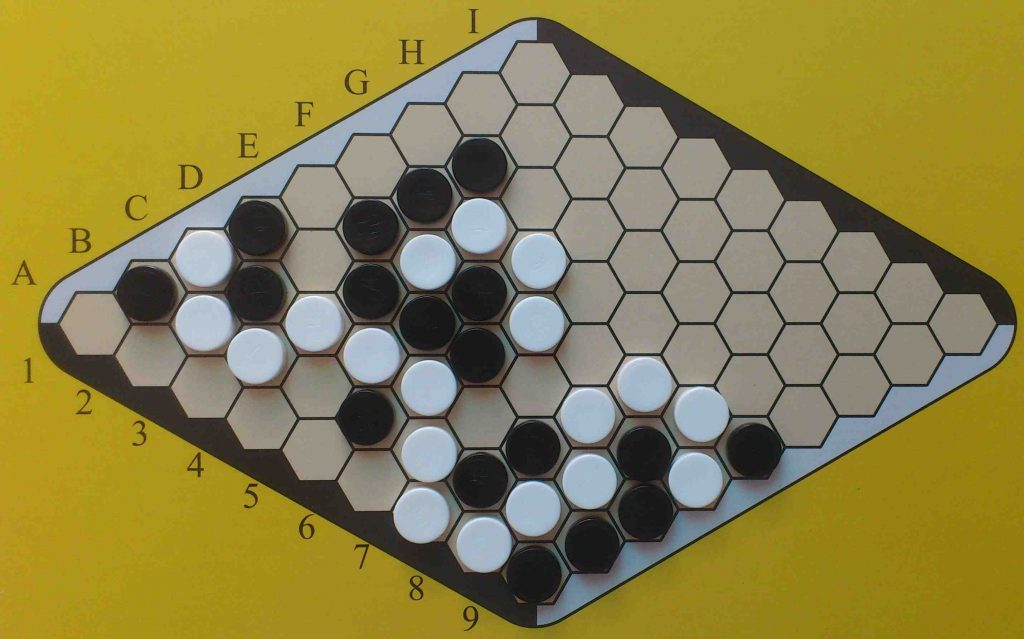
\includegraphics[width=1\textwidth]{images/JeuPlateau.jpg}
	\end{center}
	\caption{Hex}
	\label{plateau}
\end{figure}
	\newpage



Le premier joueur utilise des pièces noires et le second joueur utilise des pièces blanches.
Le but du premier joueur est de former une connexion avec les pièces du bord supérieur au bord inférieur, tandis que le second joueur essaiera de former une connexion entre le bord gauche et le bord droit. 

\begin{figure}[!h]
    \centering
    \begin{subfigure}
        \includegraphics[width=0.6\textwidth]{images/newP2.png}
    \end{subfigure}
    \caption{Tableau hexagonal 11x11 vide}
    \begin{subfigure}
        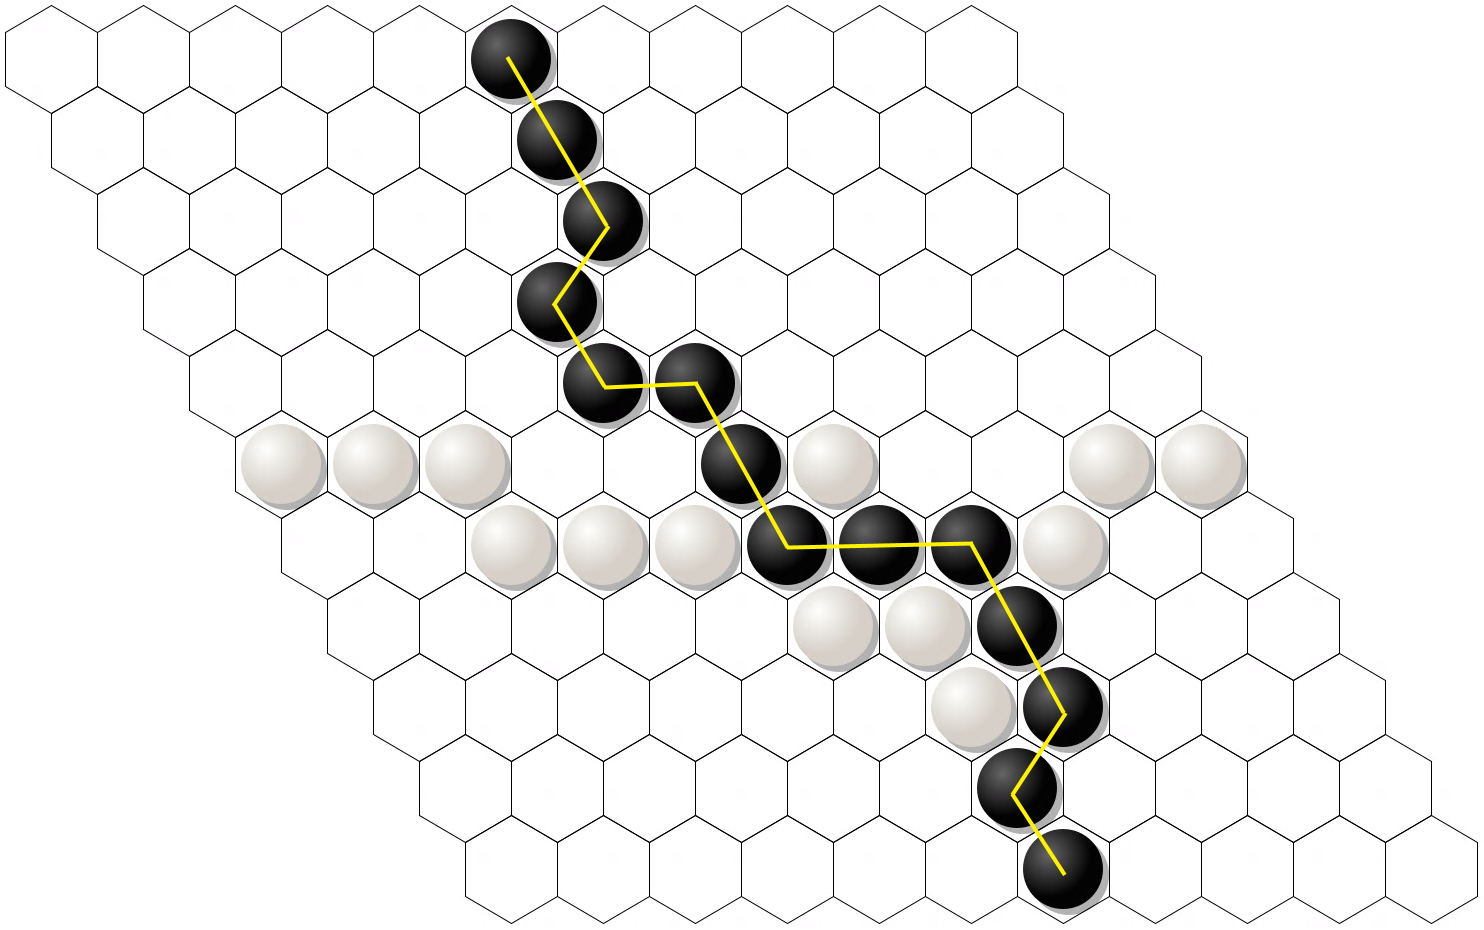
\includegraphics[width=0.6\textwidth]{images/newP1.png}
    \end{subfigure}
    \caption{Exemple d'une partie}
\end{figure}

Ici on peut observer que c'est le joueur avec les pièces noirs qui a gagné la partie.


Une partie d'Hex ne peut jamais se terminer par un match nul. En tant que tel, le seul moyen de bloquer complètement l'adversaire est de former une connexion avec ses propres pièces. La recherche d'une où des stratégies gagnantes deviennent de plus en plus difficiles lorsque la taille du plateau augmente jusqu'à des plateaux, en général la taille d'un plateau est de 14 x 14. En raison de l'avantage significatif que le premier joueur à placer sa pièce a, le jeu est couramment joué avec la règle de l'échange. Cette règle stipule qu'après que le joueur Noir est placé sa première pièce, le joueur Blanc peut choisir d'échanger cette pièce contre une pièce blanche ou pas. Le jeu se poursuit alors avec les noirs, qui sont devenus le deuxième joueur.

	
\section{\underline{Organisation}}
	Pour la répartition des tâches elle a été faite sans véritable organisation  mais nous pouvons considérons la répartition suivante:
 \\
	  celestion Mireux :
	\begin{itemize}
	\item Partie Graphique
	\item  rapport
	\end{itemize}
	Daouda TRAORE :
	\begin{itemize}
	\item Réalisation du moteur
	\item Partie Graphique
	\item  Rapport
	\end{itemize}
	  Amadou Bah :
	\begin{itemize}
	\item Réalisation du moteur
	\item Tests
	\item Rapport
	\end{itemize}
   Junior MISSOUP :
	\begin{itemize}
	\item Rapport
	\end{itemize}
	Pour la prochaine fois une meilleure organisation sera notre premier objectif, mais étant des amateurs nous avons un petit peu avancé à l'aveuglette.\\
\newpage
\subsection{\underline{Gestion du projet}}

Afin de faciliter la communication et le bon déroulement de la conception de notre jeu, divers moyens ont été mis en oeuvre.

\subsubsection{\underline{Hébergement du code}}

	Afin de faciliter la gestion du projet, nous avons utilisé à la fois \href{https://forge.info.unicaen.fr/}{la Forge} d’Unicaen qui permet de créer et d’administrer des dépôts sous Git très facilement par l’intermédiaire d’une interface web. D'ailleurs pour tous les membres l'utilisation de GIT fut une première, donc un temps d'acclimatisation et d'apprentissage nous a été nécessaire. D’autres fonctionnalités sont disponibles  sur cette plateforme comme une gestion des permissions, une visualisation des différents commits, la visualisation de l’activité du projet, etc. L'utilisation supplémentaire de \href{https://github.com/}{Github} permettait de centraliser les projets du cursus de la licence sur une seule plateforme(plus à but personnel).
	
\subsubsection{\underline{Gestionnaire de version}}

	Nous avons utilisé un gestionnaire de version afin de permettre la centralisation du code et rendre le travail en équipe de manière bien plus efficace. Nous avons opté pour Git comme gestionnaire de fichiers sans raison particulière, qui en fin de compte s'avérait être un bon choix. Sur Git  l'utilisation des branches est très facile, elle permet de faire des commits sans pour autant être connecté sur le serveur. Cela permet de faire plus de commits, qui sont enregistrés localement et de les envoyer sur le serveur en une seule fois, au moment où nous sommes sûrs que la fonctionnalité ajoutée fonctionne. Git permet également de transférer facilement son code vers un autre hébergeur en ajoutant simplement une "route" (remote), tout en conservant la totalité des commits réalisés.




\section{\underline{Conception}}
	\subsection{Arborescence du projet}
 \textbf{\underline{Jeu de Hex et bandits manchots }}:\\
	Réprésente l'espace de travail.\\
	\textbf{\underline{Rapport}}:\\
	Le répertoire contenant les différents éléments du rapport.\\
	\textbf{\underline{exe}}:\\
	Contient le jar.\\
	\textbf{\underline{bin}}:\\
	Répertoire contenant les .class.\\
	Au fur et à mesure de l'avancement le projet a pris pour arborescence la suivante \ref{abr} : \\
	\\
	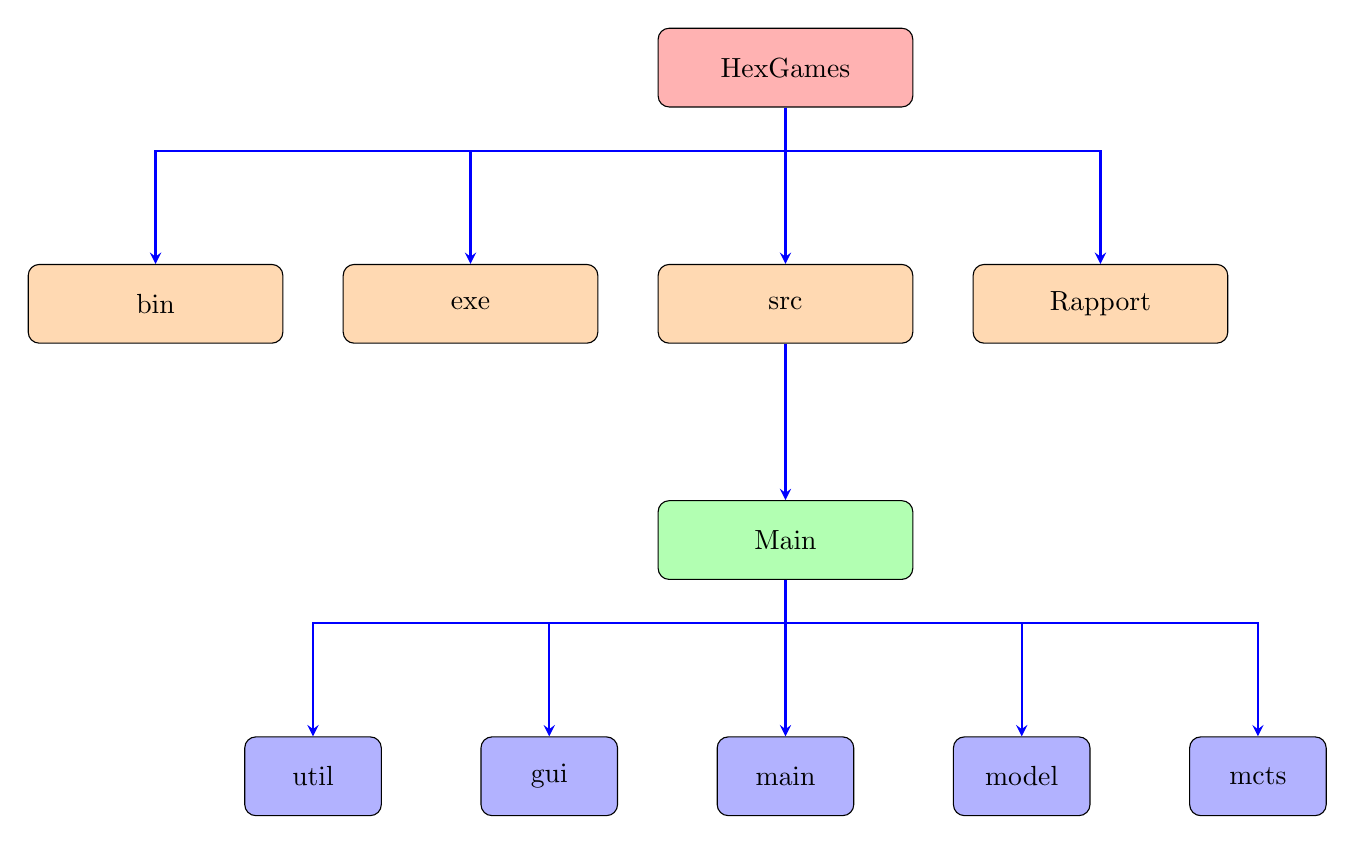
\begin{tikzpicture}[node distance=3cm]
		\node (start) [node] {HexGames} ;
		\node (Hex) [level1, below of=start] {src};
		\node (Rapport) [level1, right of=Hex, xshift = +1cm] {Rapport};
		\node (exe) [level1, left of=Hex, xshift = -1cm] {exe};
		\node (bin) [level1, left of=exe, xshift = -1cm] {bin};
		\node (src) [level2, below of=Hex] {Main};
		\node (main) [level3, below of=src] {main};
		\node (model) [level3, right of=main] {model};
		\node (mcts) [level3, right of=model] {mcts};
		\node (gui) [level3, left of=main] {gui};
		\node (util) [level3, left of=gui, xshift = 0cm] {util};
		
		\draw [arrow] (start) -- +(0,-30pt) -| (Hex);
		\draw [arrow] (start) -- +(0,-30pt) -| (exe);
		\draw [arrow] (start) -- +(0,-30pt) -| (bin);
		\draw [arrow] (start) -- +(0,-30pt) -| (Rapport);
		\draw [arrow] (Hex) -- +(0,-30pt) -| (src);
		\draw [arrow] (src) -- +(0,-30pt) -| (main);
		\draw [arrow] (src) -- +(0,-30pt) -|(gui);
		\draw [arrow] (src) -- +(0,-30pt) -| (util);
		\draw [arrow] (src) -- +(0,-30pt) -| (model);
		\draw [arrow] (src) -- +(0,-30pt) -| (mcts);
		\label{abr}
	\end{tikzpicture}

\subsection{\underline{Architecture du programme}}
	\subsubsection{\underline{Diaggramme des packages}}
	Le diagramme suivant est sa forme finale prise une fois que tous les éléments ont été correctement implémenté.\\
	
	\begin{figure}[h!]
		\begin{center}
			\includegraphics[width=1\textwidth]{images/pa.png}
		\end{center}
		\caption{Diagramme UML}
		\label{DU}
	\end{figure}
	Comme nous pouvons le voir le code source est décomposé en 5 packages avec le pattern \textbf{MVC} en plus pour une plus facile
	implémentation de l'interface graphique.
	\begin{itemize}
		\item Le package \textbf{model} constitue le moteur du jeu .
		\item Le package \textbf{gui} constitue la partie \textbf{vue + controlleur}
		\item Le package \textbf{Mcts} contient le l'agorithme de MCTS.
	\end{itemize}

	\section{\underline{Réalisation du Moteur}}
	La réalisation du moteur était la première étape que nous avions entamée et la dernière à être achevée car jusqu'au bout de multiples bugs ont dû être corrigé et de nouvelles fonctionnalités ont été ajoutées afin que les autres parties puissent fonctionner correctement.
	\subsection{\underline{Réalisation du Board}}
 \subsubsection{\underline{UML des classes}}
	\begin{figure}[h!]
		\begin{center}
			\includegraphics[width=1\textwidth]{images/ihm.png}
		\end{center}
		\caption{Diagramme UML du package tab}
		\label{tabuml}
	\end{figure}
	\begin{figure}[h!]
		\begin{center}
			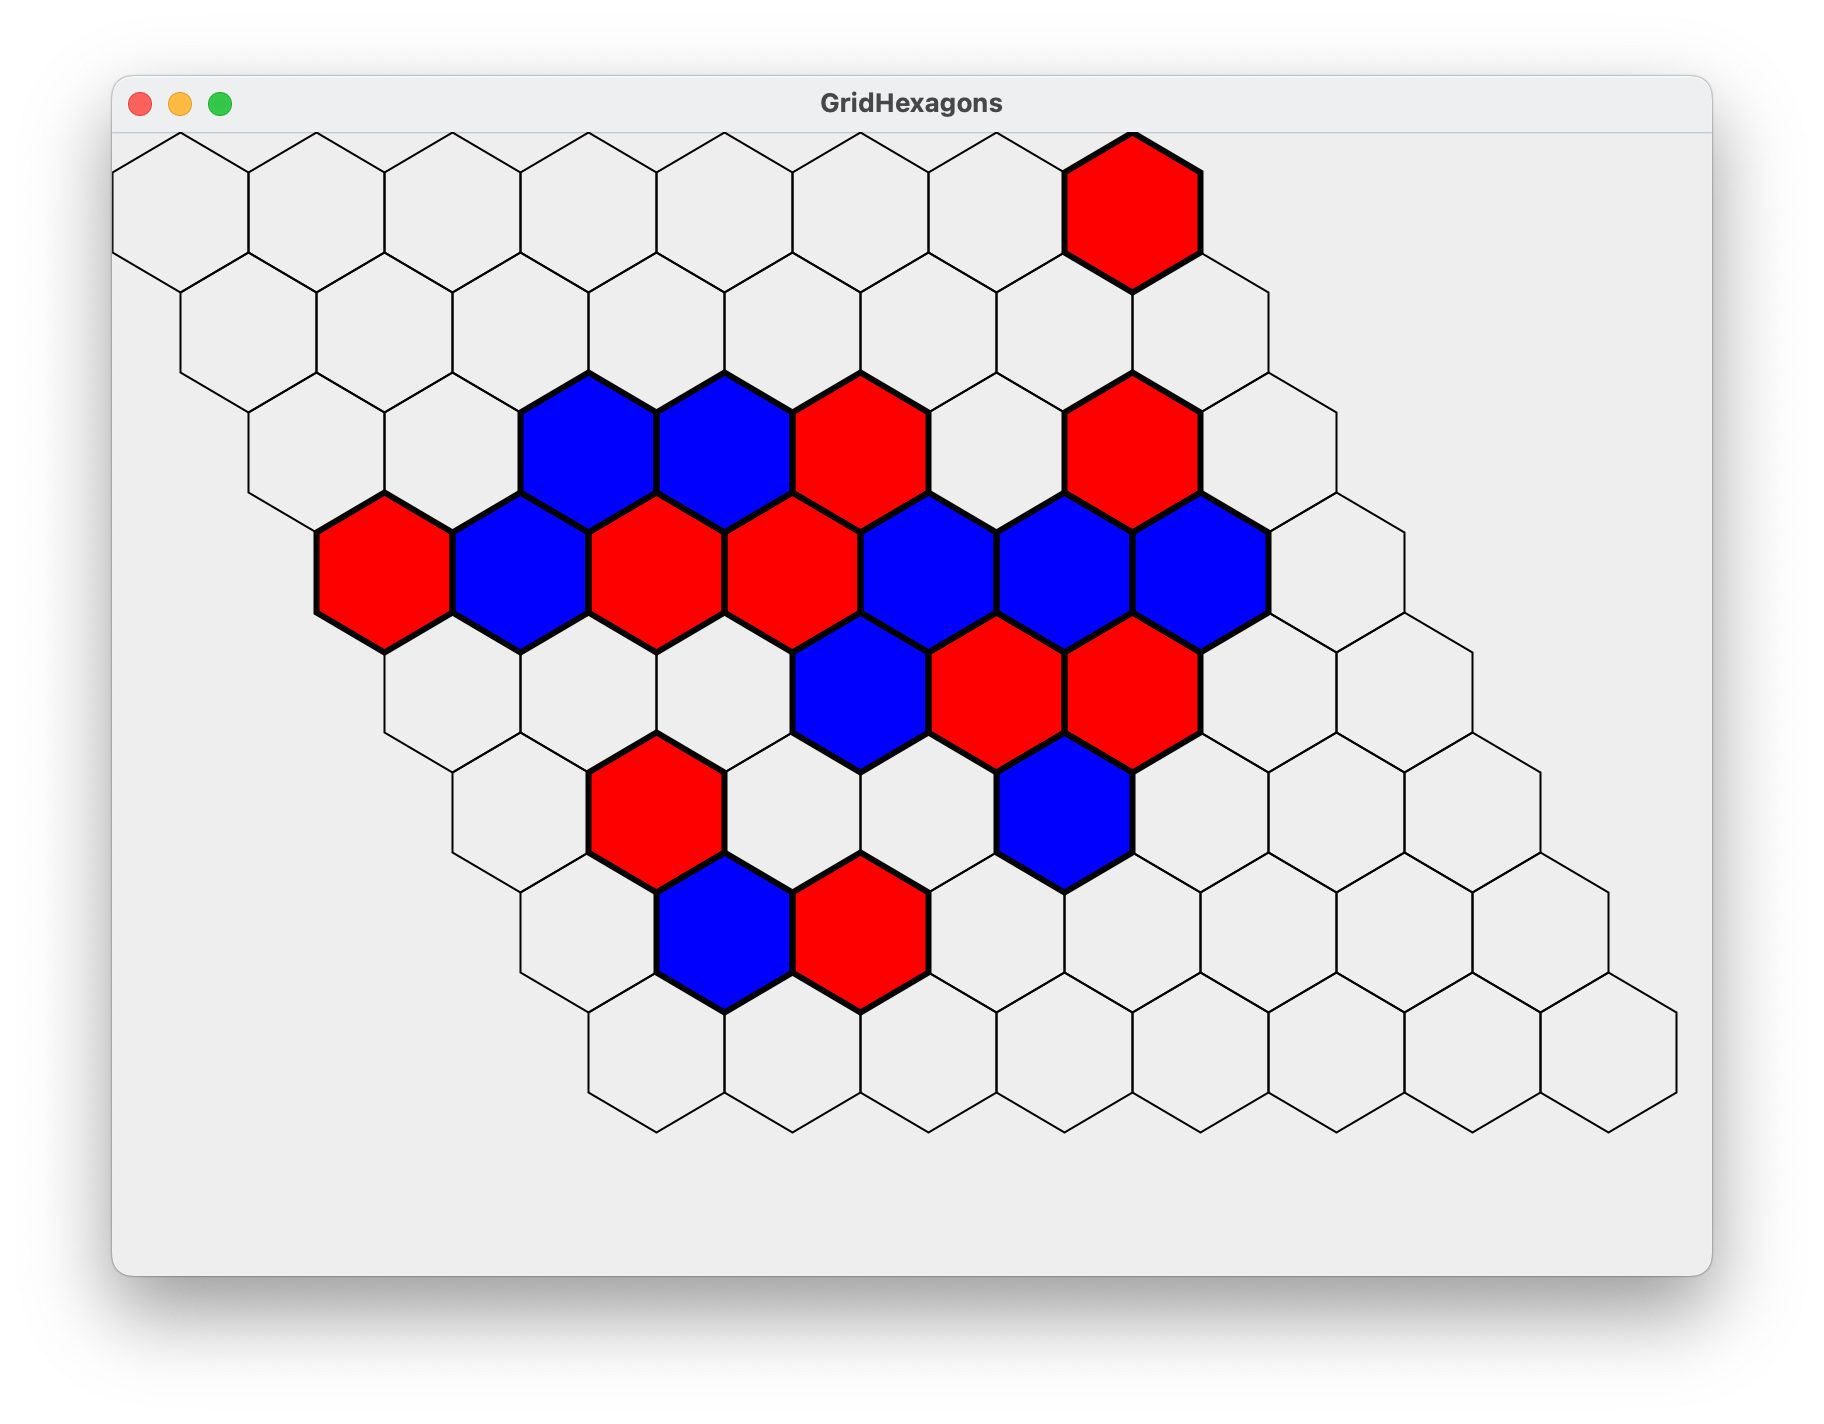
\includegraphics[width=1\textwidth]{images/Board.png}
		\end{center}
		\label{tabuml}
	\end{figure}
\newpage
	\subsubsection{\underline{Création du Plateau}}
	Pour concevoir le jeu de Hex, la première question que nous nous sommes posé à été: \textbf{comment devons-nous créer le plateau?}. 
	Le plateau de Hex est un plateau hexagonal dont les cases sont hexagonales
	\\
	Pour créer le plateau, on avait plusieurs d'idées, on  voulait d'abord partir sur une représentation en 3 dimensions qui était un peu complexe à comprendre. Après mur réflexion on s'est décidé à faire un tableau 2d avec une fonction de voisinage pour "transformer" les cases carrées des tableaux qui ont 4 voisins en case hexagonale qui en ont six. \\
	
	\subsection{\underline{Fonctionnement du moteur}}
	Une fois le plateau fait, nous nous sommes penché sur le coeur de l'application c'est-à-dire le moteur du jeu dont la majorité des fonctionnalités appartiennent à la classe \textbf{State} qui également joue le rôle de modèle dans l'architecture MVC.
	
	\subsubsection{\underline{Description}}
  \subsubsection{\underline{UML des classes}}
	\begin{figure}[h!]
		\begin{center}
			\includegraphics[width=1\textwidth]{images/mod.png}
		\end{center}
		\caption{Diagramme UML du package tab}
		\label{tabuml}
	\end{figure}
	La classe \textbf{State} donne l'état du jeu à tout instant donné. Elle initialise le jeu en créant un plateau vide. Dans la fenêtre, nous faisons apparaitre un plateau de jeu 11 x 11. Pour pouvoir placer les pions, nous avons développé certaines fonctions qui permettent de placer le pion dans une case. Concernant l’IA, pour pouvoir jouer, le programme fournit les coordonnées du coup qu'il veut réaliser, et parmi les modules créés se trouvent certaines fonctions permettant de placer le pion automatiquement avec ces coordonnées.

Le jeu repose sur de la manipulation de matrice. En effet, nous avons représenté le plateau de jeu 11 x 11 par une matrice à 11 lignes et 11 colonnes. Les éléments de cette matrice sont soit 0, 1 ou 2. 0 correspond à une case vide, 1 correspond à une case sur laquelle se trouve un pion Rouge et les pions Bleus se trouvent sur la case marquée de l’élément 2. Par exemple, si l’élément (3,4) de la matrice est 2, alors un pion bleu se trouve sur la case (3,4). Ainsi, Pour pouvoir jouer, le joueur recupere un coup dans un set de moves(\textbf{classe Move}) . Quant à l’ordinateur, il joue ses coups en fournissant à la fonction d’affichage les coordonnées du coup qu’il a sélectionné après avoir appliqué l’algorithme MCTS via la classe \textbf{MonteCarloTreeSearch} plusieurs fois (par exemple 1000 fois pour qu’il y ait assez de simulations de parties pour pouvoir donner un coup suffisamment efficace).
\\
Cependant pour déterminer si un joueur a gagné on utilise une recherche en profondeur, contrairement au parcours en largeur, lorsque l’on fait un parcours en profondeur à partir d’une case donnée, on tente d’avancer le plus loin possible dans le jeu, et ce n’est que lorsque toutes les possibilités de progression sont bloquées que l’on revient (étape de backtrack) pour explorer un nouveau chemin ou une nouvelle chaîne. Le parcours en profondeur correspond aussi à l’exploration d’un labyrinthe. Les applications de ce parcours sont peut-être moins évidentes que pour le parcours en largeur, mais le parcours en profondeur permet de résoudre efficacement des problèmes plus difficiles.Voici l'algo qu'on a implémenté
\begin{algorithm}
\KwIn{$x, y$ : position du joueur courant}
\KwIn{currentPlayer : joueur courant}
\KwOut{true si le joueur courant a gagné, sinon false}
\If{currentPlayer == PLAYER1 \textbf{and} x == rows - 1}{
    \Return true;\\
}
\ElseIf{currentPlayer == PLAYER2 \textbf{and} y == cols - 1}{
        \Return true;\\
}
visited[x][y] = true;\\
\If{GetCell(x - 1, y) == currentPlayer \textbf{and} visited[x - 1][y] == false}{
    \If{dfs(x - 1, y, currentPlayer) == true}{
        \Return true;\\
    }
}
\If{GetCell(x - 1, y + 1) == currentPlayer \textbf{and} visited[x - 1][y + 1] == false}{
    \If{dfs(x - 1, y + 1, currentPlayer) == true}{
        \Return true;\\
    }
}
\If{GetCell(x, y - 1) == currentPlayer \textbf{and} visited[x][y - 1] == false}{
    \If{dfs(x, y - 1, currentPlayer) == true}{
        \Return true;\\
    }
}
\If{GetCell(x, y + 1) == currentPlayer \textbf{and} visited[x][y + 1] == false}{
    \If{dfs(x, y + 1, currentPlayer) == true}{
        \Return true;\\
    }
}
\If{GetCell(x + 1, y - 1) == currentPlayer \textbf{and} visited[x + 1][y - 1] == false}{
    \If{dfs(x + 1, y - 1, currentPlayer) == true}{
        \Return true;\\
    }
}
\If{GetCell(x + 1, y) == currentPlayer \textbf{and} visited[x + 1][y] == false}{
    \If{dfs(x + 1, y, currentPlayer) == true}{
        \Return true;\\
    }
}
\Return false;\\
\caption{DFS pour le jeu Hex}
\end{algorithm}
\newpage

cette méthode, est une fonction récursive qui utilise la recherche en profondeur pour explorer les cellules adjacentes à une cellule donnée et vérifie si elles sont de la même couleur que le joueur en cours. La méthode prend deux paramètres: les coordonnées de la cellule actuelle (x, y) et l'identifiant du joueur actuel (PLAYER1 ou PLAYER2). La méthode marque chaque cellule visitée en utilisant un tableau \textbf{visited} et s'arrête et renvoie \textbf{true} si elle trouve une cellule qui correspond à la couleur du joueur qui forme une connexion ininterrompue jusqu'à la rangée opposée.
\begin{algorithm}
\SetAlgoLined
\KwIn{currentPlayer : joueur courant}
\KwOut{true si le joueur courant a gagné, sinon false}
boolean gameOver = false;\\
int y = 0, x = 0;\\
int end = (currentPlayer == PLAYER1 ? cols : rows);\\
\For{int i = 0; i < cols; i++}{
    \For{int j = 0; j < rows; j++}{
        visited[i][j] = false;\\
    }
}
\For{int i = 0; i < end; ++i}{
        \If{GetCell(x, y) == currentPlayer \textbf{and} dfs(x, y, currentPlayer) == true}{
            gameOver = true;\\
            \textbf{break};\\
        }
        \If{currentPlayer == PLAYER1}{
                y++;\\
        }
        \Else{
            x++;\\
        }
}
\Return gameOver;\\
\caption{fonction isOver}
\end{algorithm}
\newpage
La  méthode, \textbf{isOver}, prend également un paramètre \textbf{currentPlayer} et vérifie si le joueur a gagné la partie en appelant la méthode \textbf{dfs} pour chaque cellule de la première colonne ou ligne en fonction du joueur actuel. Elle parcourt chaque cellule de la première colonne ou ligne selon le joueur actuel et vérifie si elle est de la même couleur que le joueur. Si la méthode \textbf{dfs} renvoie \textbf{true} pour l'une de ces cellules, cela signifie que le joueur a gagné et la méthode renvoie \textbf{true}. Sinon, la méthode renvoie \textbf{false}.
\section{\underline{Recherche arborescente de Monte Carlo}}
 \subsection{\underline{Recherche arborescente }}
Dans un plateau Hex de taille n × n, la configuration de départ vide a n × n mouvements possibles. Chaque coup donne une nouvelle configuration unique des pièces sur l'échiquier. Ces configurations peuvent être organisées hiérarchiquement dans une structure arborescente. La configuration de départ était le nœud
 racine, chaque position de l'échiquier atteignable à partir de cette position sera des enfants rattachés au nœud. Cet arbre se poursuit jusqu'aux nœuds terminaux, c'est-à-dire les positions où le jeu est terminé. La figure ci-dessous montre comment un arbre de 2 × 2 Hex qui se développe.

\begin{figure}[h!]
		\centering
		\includegraphics[width = 1\textwidth]{images/treeSearch.png}
		\caption{Structure arborescente  2×2 Hex}
		\label{eq1}
	\end{figure}
 
La recherche arborescente est une méthode de recherche d'un arbre à partir d'une position de départ donnée, afin de trouver des positions de conseil bénéfiques plus bas dans l'arbre. Certaines stratégies de recherche arborescente pour explorer l'arbre sont la recherche en largeur d'abord et la recherche en profondeur d'abord.
	\subsection{\underline{Algorithme de recherche arborescente de Monte Carlo}}

   L’algorithme Monte-Carlo Tree Search (MCTS), ou l’algorithme UCB1, est un algorithme
d’apprentissage par renforcement qui consiste en une recherche heuristique pour
permettre une certaine prise de décision. C’est un procédé qui cherche à faire une
balance entre l’exploration, c’est-à dire-trouver des actions potentiellement profitables et
l’exploitation, qui consiste à choisir la meilleure action empirique le plus souvent possible.
Ceci dans le but de prendre empiriquement la meilleure action aussi souvent que
possible. Cette méthode a pour support l’arbre présenté dans la section précédente.
Dans cet algorithme chaque noeud (ou feuille) et la racine possèdent certaines quantités
exploitées par l’algorithme qui interviennent dans la formule suivante :

\begin{equation}
  UCB1(N,c) = \frac{\omega}{n} + c\sqrt{\frac{\ln{(N)}}{n}}
\end{equation}
avec N le nombre de parties totales simulées. Ces
quantités sont :
\begin{itemize}
	\item $ n_i $ : le nombre  de fois où le noeud i a été visité
	\item{ $ \omega_i $ :le nombre de parties remportées par la couleur du noeud i}
	\item la valeur de UCB1
\end{itemize}
L’algorithme MCTS est composé de 4 étapes :
\begin{itemize}
	\item Sélection
	\item Expansion
	\item Simulation
    \item Backpropagation
\end{itemize}
 La \textbf{sélection} consiste à sélectionner une série de noeuds depuis la racine jusqu’à
atteindre une feuille. Cette sélection s’effectue en gardant un compromis entre le choix
d’un noeud qui a été prouvé comme prometteur (ou exploitation qui est représentée par 
\begin{math} 
\frac{\omega}{n}
\end{math}
dans la formule) et le choix d’un nouveau noeud qui paraît prometteur (ou exploration
correspondant à 
\begin{math}
\sqrt{\left(\frac{\ln{(N)}}{n}}\right)
\end{math}
)
\\

Lors de l’\textbf{expansion}, on parcourt en respectant la sélection jusqu’à atteindre une feuille.
Si cette feuille n’est pas finale (si elle ne correspond pas à une configuration finale de jeu)
alors en suivant les règles du jeu on ajoute autant de noeuds fils à cette feuille que de
coups possibles.
\\
La \textbf{simulation} consiste à terminer la partie en partant de la configuration donnée par là
feuille.

Enfin la back \textbf{propagation} modifie les données des noeuds en remontant la branche
concernée. Ce procédé consiste à incrémenter de 1 le nombre de visites des noeuds sur
la branche et à incrémenter de 1 la donnée $ \omega $ qui correspond au nombre de parties
remportées par la couleur du noeud ($\omega_racine $ est incrémenté de 1 dans tous les cas).
a difficulté principale est la phase de sélection. Pour construire l’arbre, il faut choisir un
noeud fils tout en maintenant le compromis entre exploitation et exploration. Ce
compromis se traduit par le choix du noeud k qui maximise la formule UCB1. Voici ci-
dessous le résumé de l’algorithme MCTS :
	\begin{figure}[h!]
		\centering
		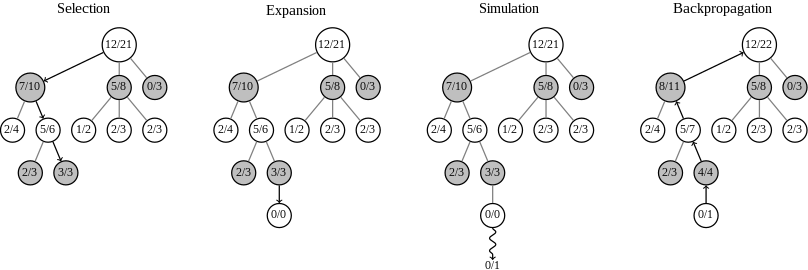
\includegraphics[width = 1\textwidth]{images/MCTS_(French).svg.png}
		\caption{Formule de calcul du coût}
		\label{eq1}
	\end{figure}

\newpage
\begin{figure}[h!]
		\centering
		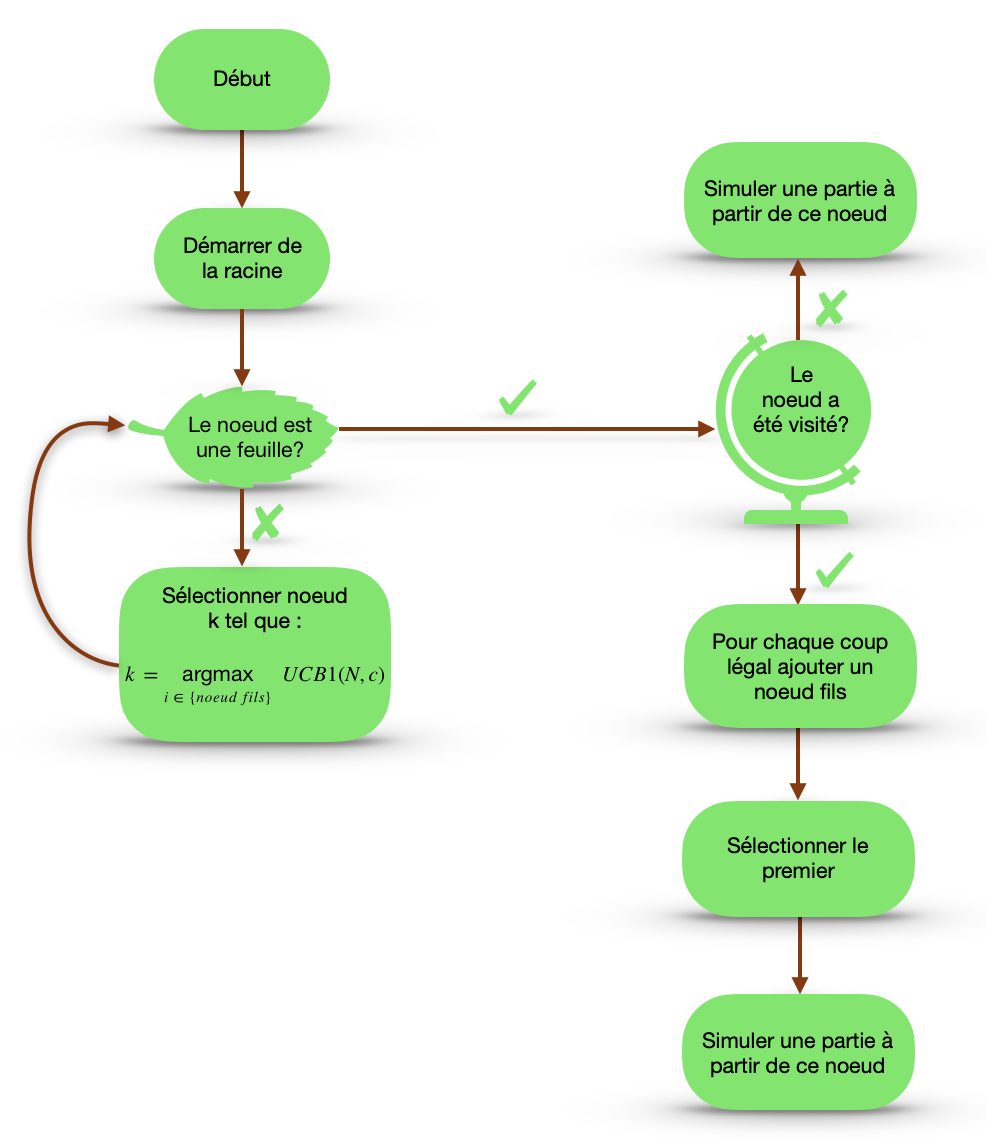
\includegraphics[width = 1\textwidth]{images/mcts.png}
		\caption{Schéma de MCTS}
		\label{eq1}
	\end{figure}
Lorsque l’on ajoute un noeud fils par coup possible on sélectionne le premier noeud pour
simuler la partie. Cette règle provient du fait que le nombre de visites de chacun de ces
noeuds est nul ce qui implique que chaque noeud est évalué en l’infini par la formule
UCB1. La règle devient alors choisir le noeud par ordre numérique.

\subsection{Exemple}
Nous allons donner un exemple d’application de l’algorithme. Dans cet exemple, on
pourra construire un arbre à deux niveaux.
\begin{figure}[h!]
		\centering
		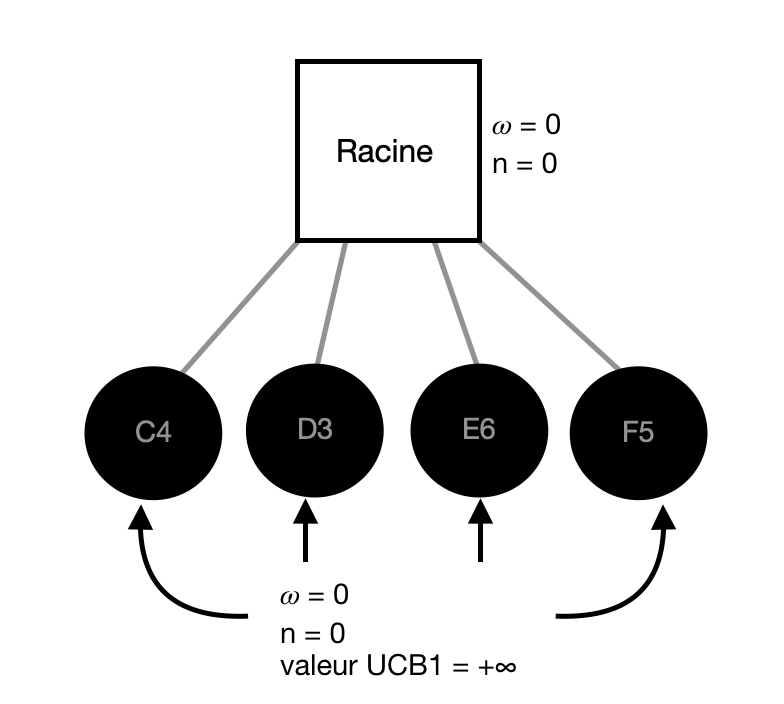
\includegraphics[width = 1\textwidth]{images/exem1.png}
		\caption{Arbre de début de jeu}
		\label{eq1}
	\end{figure}
	\newpage
On applique l’algorithme de MCTS. Les noirs commencent à jouer. La racine à ce
moment est une feuille. Les noirs peuvent jouer sur 4 cases, on ajoute alors 4 noeuds à la
racine. Tous ces noeuds possèdent les mêmes données alors on choisit le premier
noeud. Comme ce noeud est une feuille qui n’a pas été visitée, on simule la partie entière.
On suppose que les noirs ont gagné cette partie. On procède alors maintenant à la
backpropagation et on met à jour les données du noeud sélectionné. Ainsi $ \omega_{c4} = 1 , n_{c4} = 1 $ de meme que $ \omega_{racine} =1  et n_{racine} = 1 $.Lors des 3 itérations suivantes, les noeuds D3, E6
et F5 seront sélectionnés et mis à jour car ils n’avaient pas encore été visités (ainsi leur
valeur UCB1 était infinie d’où leur choix). On suppose que ces trois simulations
aboutissent à des parties perdues par les noirs. À ce stade, les 4 noeuds ont été visités
donc lors de la cinquième itération on utilise la maximisation de la formule UCB1 pour
choisir le noeud. C’est donc le noeud C4 qui maximise la formule.

\begin{figure}[h!]
		\centering
		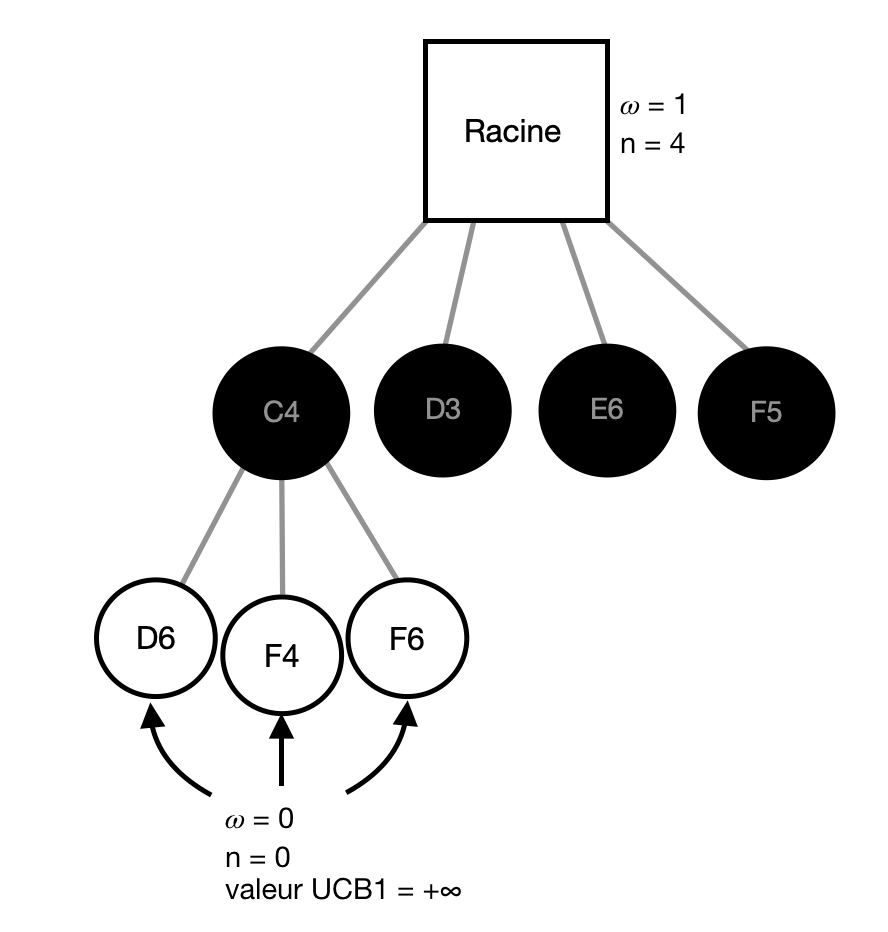
\includegraphics[width = 1\textwidth]{images/exem2.png}
		\caption{cinquième itération de MCTS}
		\label{eq1}
	\end{figure}
\newpage
 Le noeud C4 a été sélectionné, c’est une feuille qui a déjà été visitée donc on lui ajoute 3
noeuds fils qui correspondent aux coups légaux disponibles pour les blancs. On
sélectionne alors le premier (D6) et on simule la partie. On aboutit à une victoire pour les
blancs alors $ \omega_{D6} = 1 et n_{D6} = 1 $.Et ainsi de suite.
\subsubsection{\underline{UML}}
	\begin{figure}[ht!]
		\centering
		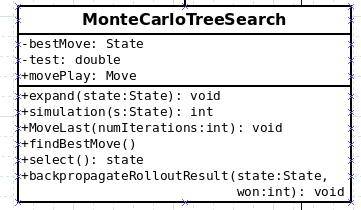
\includegraphics[width = 0.8\textwidth]{images/diaAlgo.png}
		\caption{UML du package Algo}
		\label{eq1}
	\end{figure}
\newpage
\subsection{\underline{Implémentation par rapport à notre Jeu de Hex}}
L'implémentation de MCTS s'est faite en 4 étapes comme nous l'avions précisé un peu plus tôt, mais on a une cinquième étape qui nous sert de d'un genre de fonction auxiliaire .cette fonction utilise nos 4 etapes  pour simuler plusieurs parties aléatoires à partir du nœud racine et utilise l'information obtenue pour déterminer le meilleur coup à jouer.
Les algorithmes suivants sont directement inspiré de ceux présents sur internet, les refernces sont bien données.
\begin{algorithm}
\SetAlgoLined
\DontPrintSemicolon
\KwIn{numIterations : nombre d'itérations}
\KwResult{Le meilleur coup à jouer }

\For{$i \gets 1$ \KwTo $numIterations$}{
    nodePromise $\gets$ select(rootNode);\\
    won $\gets$ simulation(nodePromise);\\
    backpropagateRolloutResult(nodePromise, won);\\
}

victories $\gets 0$;\\;
\For{child $\in$ rootNode.getChildren()}{
    \If{child.getVictories() $\geq$ victories}{
            bestMove $\gets$ child;\\
            movePlay $\gets$ bestMove.getLastMove();\\
            victories $\gets$ child.getVictories();\\
    }
}

\caption{findBestMove(numIterations)}
\end{algorithm}
\subsection{Expérimentation}
Lors de la présentation de la méthode, nous avons précisé qu'on utilisait une heuristique qui est le UCB(Upper Confident Bounded).\\
Est-ce que la recherche arborescente de Monte-Carlo vaut la peine d’être implémentée?\\
Quels sont les paramètres de l'algorithme MCTS que nous pourrions ajuster pour améliorer les performances de l'agent de jeu ?\\
Comment pourrions-nous évaluer les performances de l'agent de jeu sur le jeu de Hex ? \\
Est-ce plus efficace qu’un jeu aléatoire?


\begin{figure}[h!]
		\centering
		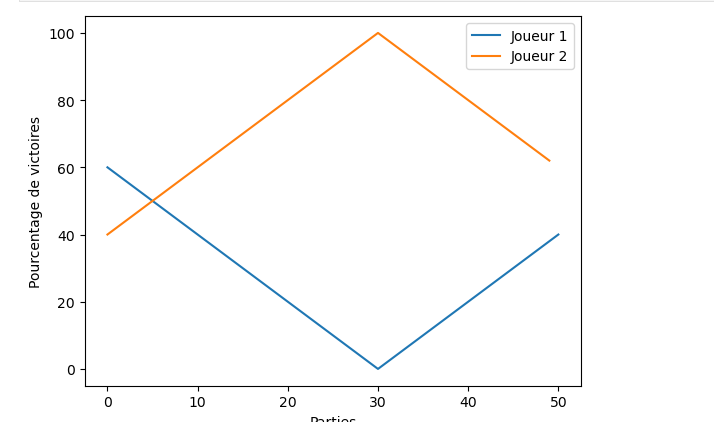
\includegraphics[width = 1\textwidth]{images/exP2.png}
		\caption{}
		\label{eq1}
\end{figure}
\\
Pour initialiser mon expérience nous voulions être d'accord que lorsque plus le budget est grand mieux sont les performances de  l'algorithme.
sur la figure ci-dessus on a le joueur 1 et le joueur 2 qui jouent avec le même budget(1000).
Et on remarque ils ont presque le  même taux de victoires, en effet pour le joueur 1 on remarque plus de victoires de son coté, c'est normal vu que c'est le premier qui commence à jouer à chaque fois à ne pas oublier sur le jeu d'hex le joueur qui commence en premier à un avantage.

\begin{figure}[h!]
		\centering
		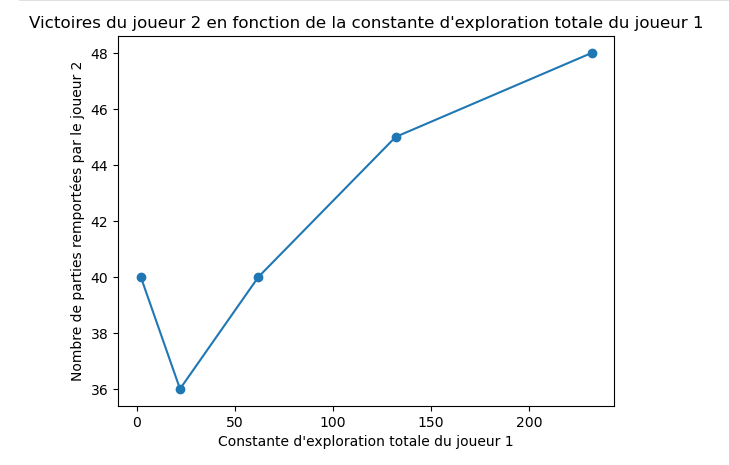
\includegraphics[width = 1\textwidth]{images/exp1.png}
		\caption{}
		\label{eq1}
	\end{figure}
 \\
 On remarque sur la figure  que le joueur 2 a gagné plus souvent que le joueur 1 lorsqu'on a augmenté la constante d'exploration du joueur 1 à 100 tandis que le joueur 2 est resté à une constante d'exploration de 2, cela peut prouver que le joueur 1 a exploré davantage de coups que le joueur 2. Bien que cela puisse sembler avantageux, explorer davantage de coups ne garantit pas toujours la victoire, car le choix des coups explorés peut également affecter le résultat du jeu.Pour c=0, on a un taux de victoire maximal pour le joueur 1, cela signifie que la recherche de l'arbre de recherche se concentrera uniquement sur l'exploitation des nœuds qui ont la meilleure estimation de la probabilité de gagner, sans prendre en compte l'exploration de nouvelles options qui pourraient être prometteuses à long terme.
\subsection{\underline{Problèmes rencontés}}
	Durant la mise en place de l'interface graphique, Cette partie du projet nous a été particulièrement difficile, nous avons
trouvé en open source une classe « Hexagon » qui compose  notre fichier. En
effet, nous avons compris comment elle fonctionnait et nous avons alors pu l’enrichir de
nos propres besoins en fonction.
	\\
    Cependant dans l'implementation de l'algorithme on a eu plusieurs dysfonctionnements qui a duré plusieurs séances de Tp. Une fois de plus le problème semblait incompréhensible car nous l'avions correctement implémenté mais le souci était chaque fois le premier joueur qui jouait gagnait  quel que soit le budget attribué. Une fois de plus est venu à la rescousse notre chargé de Tp qui après avoir revu notre code nous a faits savoir que dans notre implementation  les deux joueurs jouaient le même arbre de recherche et ainsi ça pouvait arriver qu'un joueur qui n'explore pas un noeud déjà visité par son adversaire.
    \\
    
	Pour résoudre le problème notre chargé de Tp nous a exposé plusieurs idées, toutes éventuellement  intéressantes  mais la plupart des idées allaient nous pousser à refaire le modèle ce qui nous semblait un peu tard, il y avait pas beaucoup de temps pour terminer le projet et on s'est tourné vers une option qui était nous sauvait la vie. Cette option était de faire une copie profonde de notre state initial et de le partager aux deux joueurs et après se mettre à jour plus tard le deuxième joueur qui jouera au deuxième tour. Qui fut une première car jusque-là nous n'avions jamais considéré cette éventualité.
 \\
 
	La liste de problèmes rencontrés durant ce projet étant extrêmement longue nous nous limiterons à ces deux qui furent le plus problématique.
	
	\newpage
	\section{\underline{Conclusion}}
	\subsection{\underline{Avis Général}}
	Ce projet était très intéressant. Nous ne connaissions pas le jeu de hex auparavant et c'était intéressant de se pencher, 
	sur les règles de ce jeu et de le recréer afin de pouvoir y jouer autrement que sous forme physique.\\
	Ce projet nous aura permis de beaucoup apprendre et de nous améliorer.
	
	\subsubsection{\underline{Eléments à améliorer}}
	Bien que tout ce qui a été demandé dans le sujet a été rempli, pas mal de choses restent quand même à améliorer mais faute de 
	temps et du nombre de projets ont fini en ce fin semestre tout ce que l'ont souhaité n'a pas pu être accompli.
	Par exemple;
	\begin{itemize}
 		\item L'implémentation de l'optimisation RAVE(Rapid Action Value Estimation).
		\item Amélioreration de  l'interface graphique, car l'interface finale est très basique.
		\item Rajouter d'autres fonctionnalités comme pouvoir jouer par soi-même.
		\item faire des tests comparant différents types d'algorithmes.
	\end{itemize}

	\newpage


 

 \bibliographystyle{plain}
\nocite{*}
\bibliography{bibliography} 

\section{Annexes}
\subsection{Code informatique }
voici le code de la classe MonteCarloTreeSearch :

\begin{figure}[!h]
    \centering
    \begin{subfigure}
        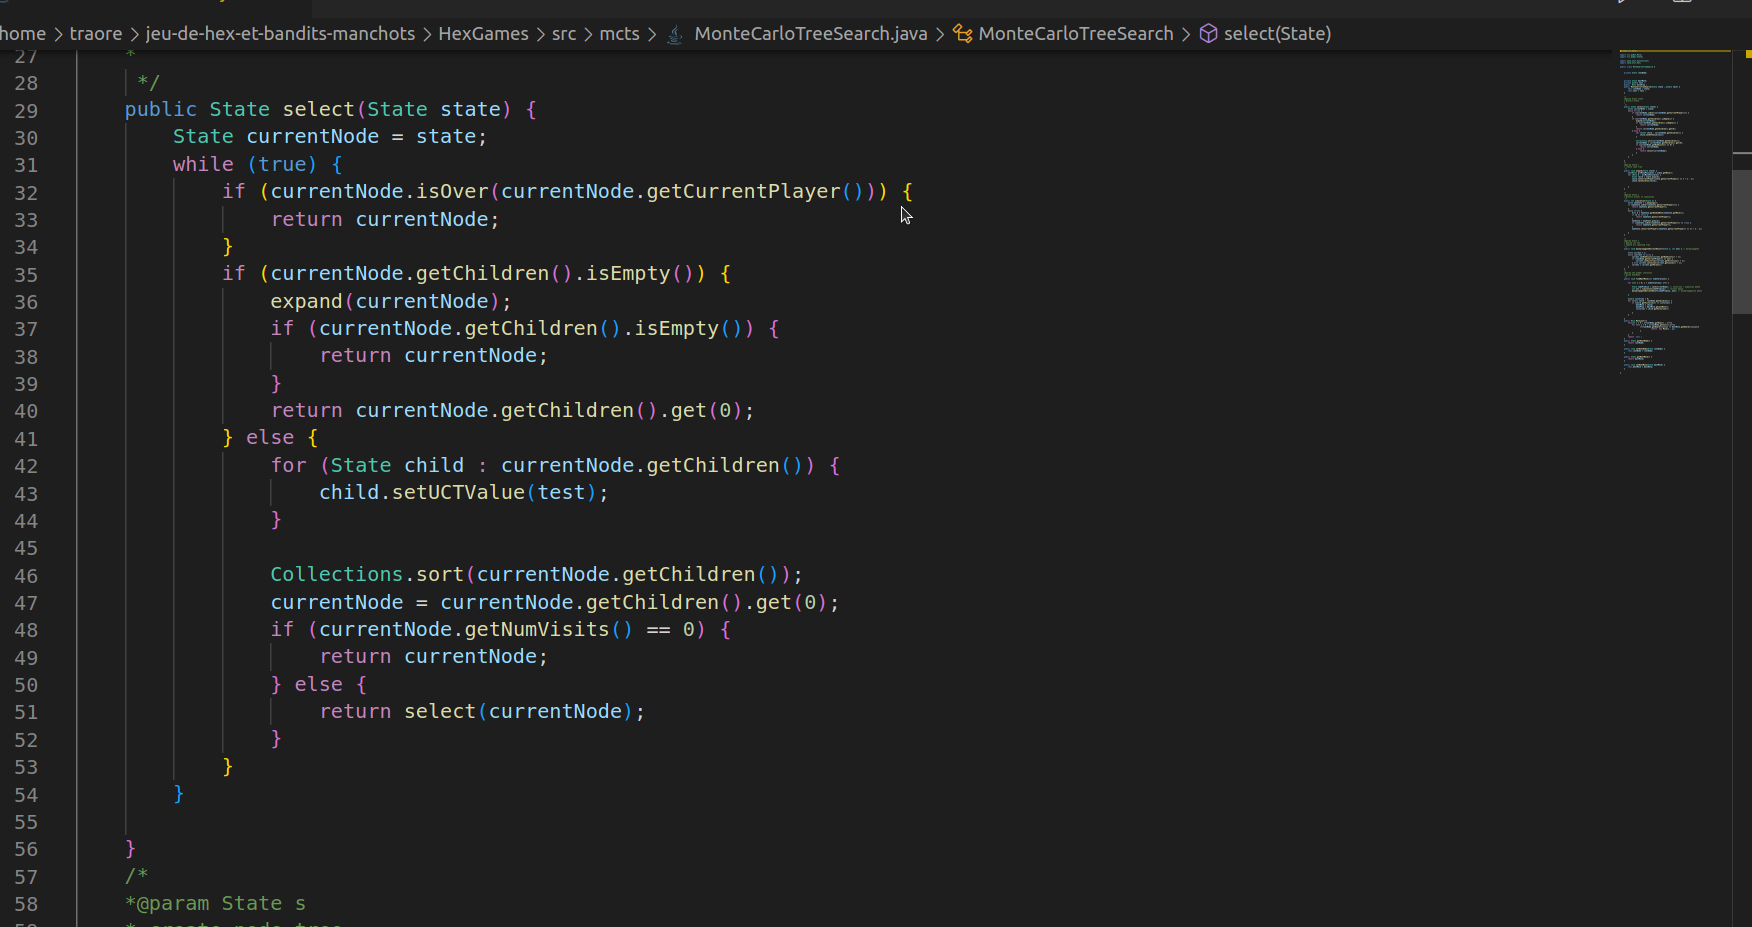
\includegraphics[width=1\textwidth]{images/select.png}
    \end{subfigure}
    \begin{subfigure}
        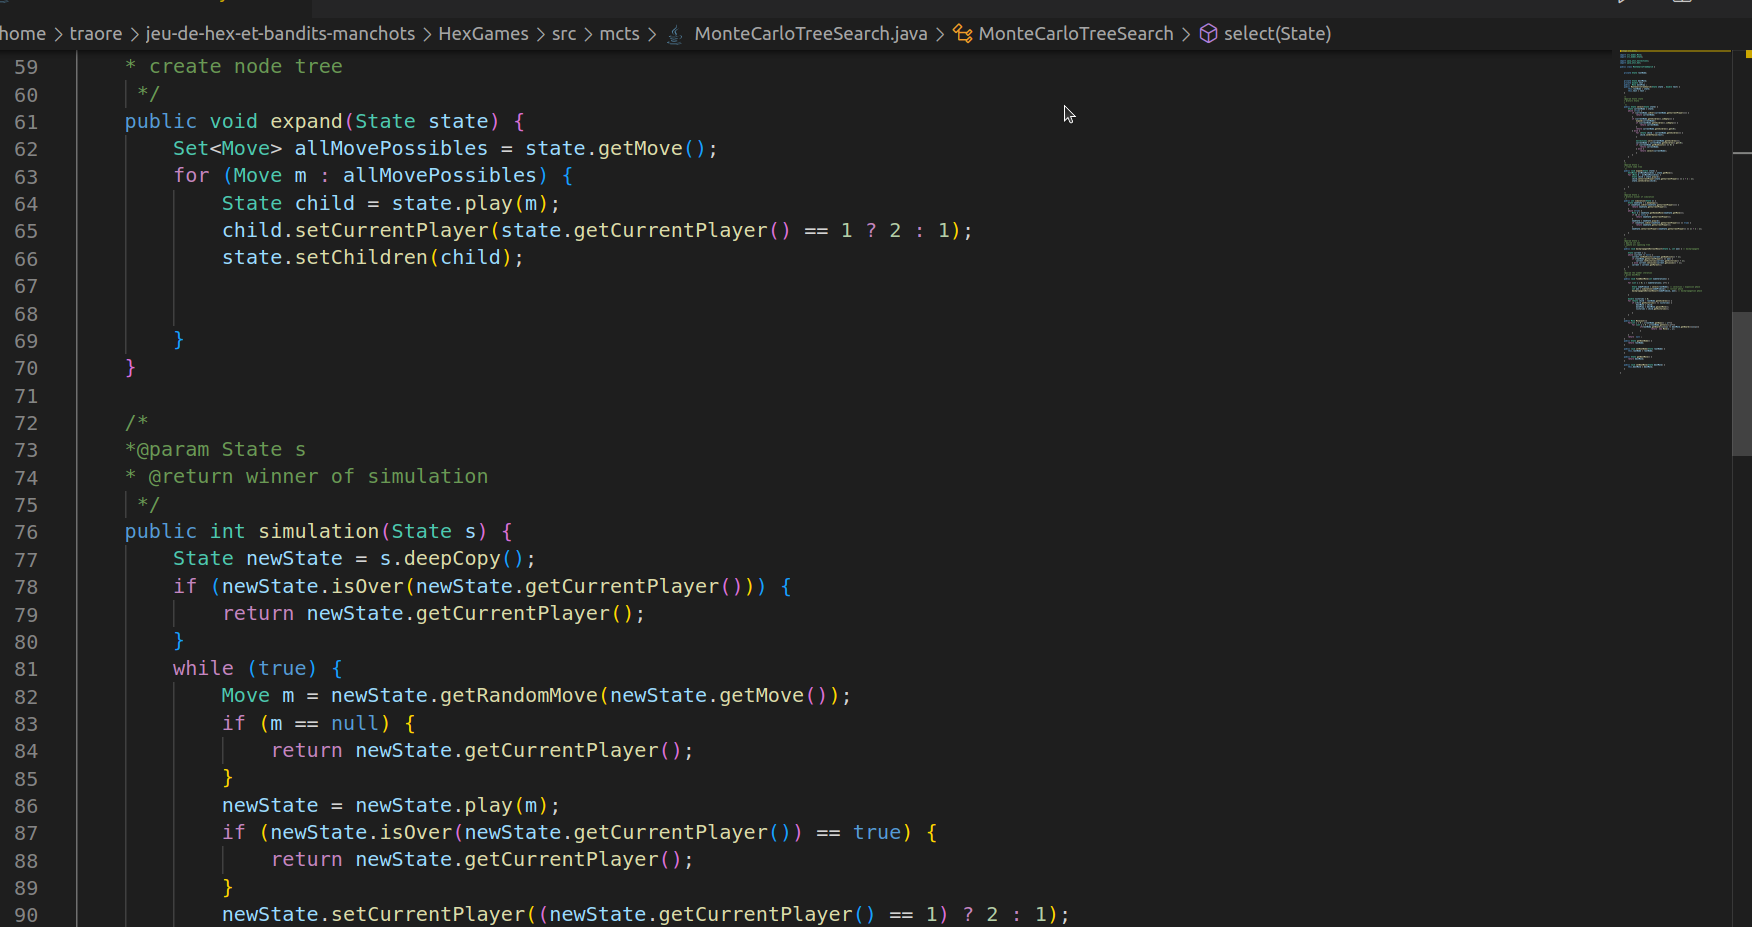
\includegraphics[width=1\textwidth]{images/sim.png}
    \end{subfigure}
     \begin{subfigure}
        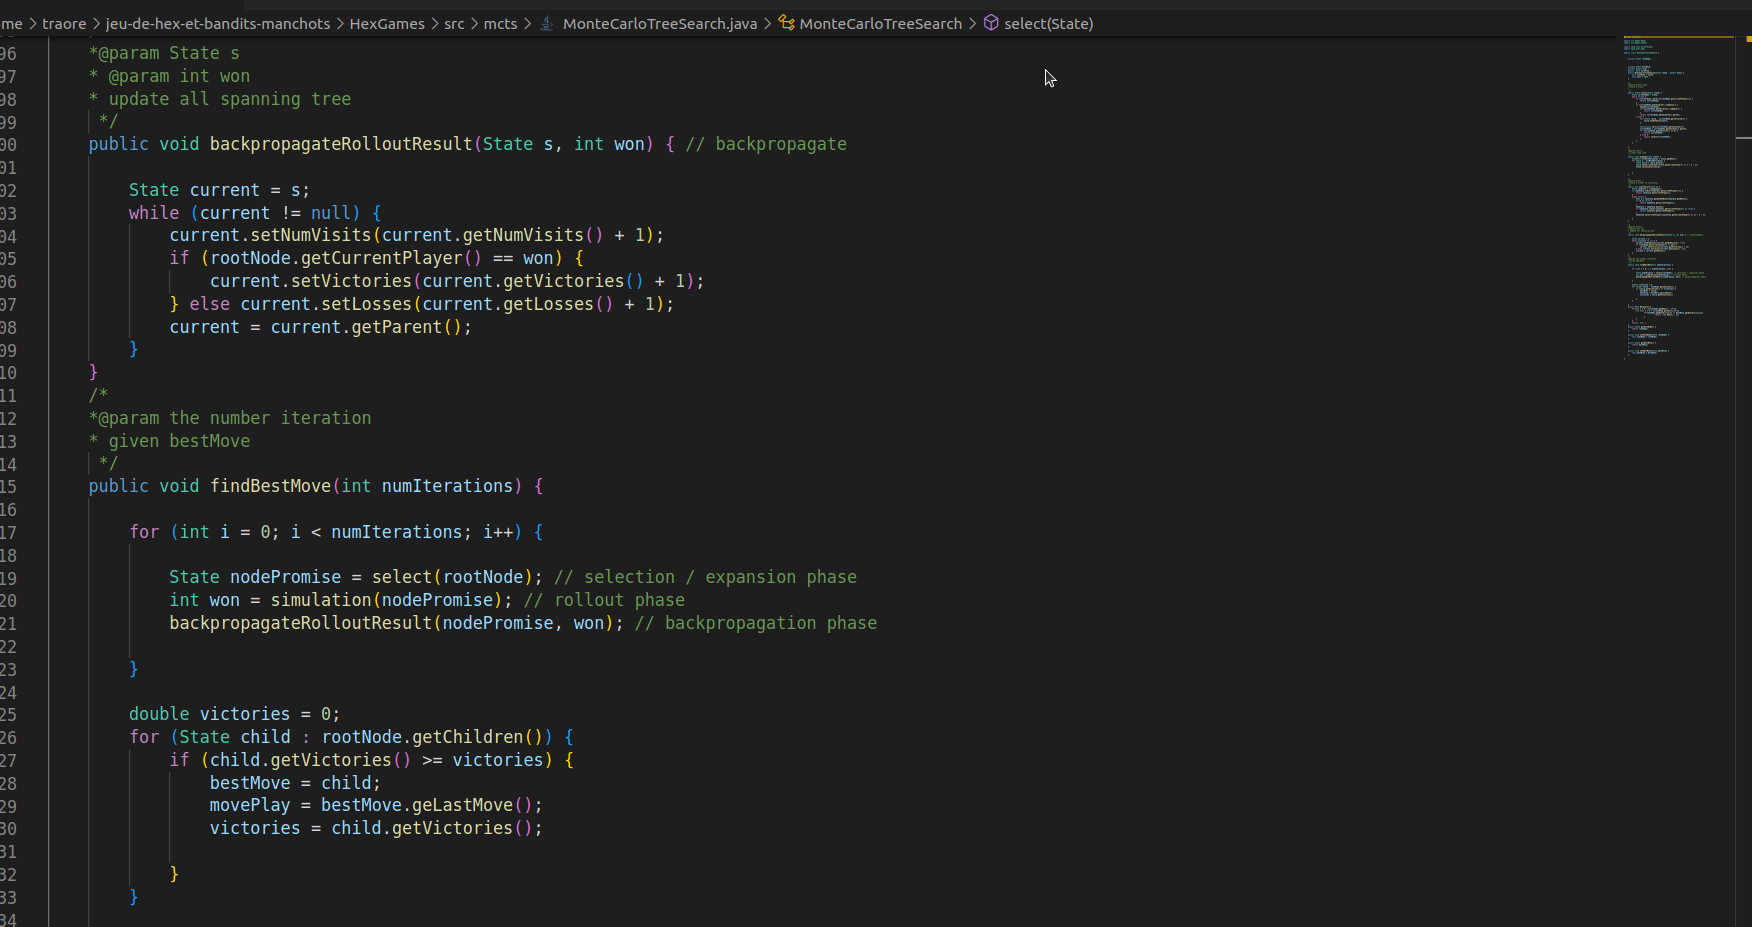
\includegraphics[width=1\textwidth]{images/back.png}
    \end{subfigure}
  
\end{figure}
\end{document}
